\let\negmedspace\undefined
\let\negthickspace\undefined
\documentclass[journal]{IEEEtran}
\usepackage[a5paper, margin=10mm, onecolumn]{geometry}
%\usepackage{lmodern} % Ensure lmodern is loaded for pdflatex
\usepackage{tfrupee} % Include tfrupee package

\setlength{\headheight}{1cm} % Set the height of the header box
\setlength{\headsep}{0mm}  % Set the distance between the header box and the top of the text

\usepackage{float}
\usepackage{gvv-book}
\usepackage{gvv}
\usepackage{cite}
\usepackage{amsmath,amssymb,amsfonts,amsthm}
\usepackage{algorithmic}
\usepackage{graphicx}
\usepackage{textcomp}
\usepackage{xcolor}
\usepackage{txfonts}
\usepackage{listings}
\usepackage{enumitem}
\usepackage{mathtools}
\usepackage{gensymb}
\usepackage{comment}
\usepackage[breaklinks=true]{hyperref}
\usepackage{tkz-euclide} 
\usepackage{listings}
\usepackage{gvv}                                        
\def\inputGnumericTable{}                                 
\usepackage[latin1]{inputenc}                                
\usepackage{color}                                            
\usepackage{array}                                            
\usepackage{longtable}                                       
\usepackage{calc}                                             
\usepackage{multirow}                                         
\usepackage{hhline}                                           
\usepackage{ifthen}                                           
\usepackage{lscape}
\usepackage{tikz}
\usepackage{float}
\begin{document}

\bibliographystyle{IEEEtran}
\vspace{3cm}

\title{2020-EE- 1-13}
\author{EE24BTECH11016 - DHWANITH M DODDAHUNDI}

% \maketitle
% \newpage
% \bigskip
{\let\newpage\relax\maketitle}

\renewcommand{\thefigure}{\theenumi}
\renewcommand{\thetable}{\theenumi}
\setlength{\intextsep}{10pt} % Space between text and floats

\begin{enumerate}
\item This book, including all its chapters, \underline{\hspace{1cm}}interesting. The students as well as the instructor \underline{\hspace{1cm}} in agreement about it.
\begin{enumerate}
    \item is, was
    \item are, are
    \item is, are
    \item were, was
\end{enumerate}
\item People were prohibited \underline{\hspace{1cm}} their vehicles near the entrance of the main administrative building.
\begin{enumerate}
    \item to park
    \item from parking
    \item parking 
    \item to have parked
\end{enumerate}
\item Select the word that fits the analogy: \\
Do : Undo :: Trust :\underline{\hspace{1cm}}
\begin{enumerate}
    \item Entrust
    \item Intrust
    \item Distrust
    \item Untrust
\end{enumerate}
\item Stock markets \underline{\hspace{1cm}} at the news of the coup.
\begin{enumerate}
    \item poised
    \item plunged
    \item plugged
    \item probed
\end{enumerate}
\item If $P,Q,R,S$ are four individuals, how many teams of size exceeding one can be formed, with $Q$ as a member?
\begin{enumerate}
    \item 5
    \item 6
    \item 7
    \item 8
\end{enumerate}
\item Non-performing assets (NPAs) of a bank in India is defined as an asset, which remains unpaid by the borrower for a certain period of time in terms of interest, principal or both. Reserve Bank of India (RBI) has changed the definition of NPA thrice during 1993-2004, in terms of the holding period of loans.The holding period was reduced by one quarter each time. In 1993, the holding period was four quarters (360 days). \bigskip
Based on the above paragraph, the holding period of loans in 2004 after the third revision was \underline{\hspace{1cm}} days.
\begin{enumerate}
    \item 45
    \item 90
    \item 135
    \item 180
\end{enumerate}
\item Select the next element of the series: Z, WV, RQP,\underline{\hspace{1cm}}
\begin{enumerate}
    \item LKJI
    \item JIHG
    \item KJIH
    \item NMLK
\end{enumerate}
\item In four-digit integer numbers from 1001 to 9999, the digit group "37" (the same sequence) appears \underline{\hspace{1cm}} times.
\begin{enumerate}
    \item 270
    \item 279
    \item 280
    \item 299
\end{enumerate}
\item Given a semicircle with O as the center, as shown in the figure, the ratio $\frac{\overline{AC}+\overline{CB}}{\overline{AB}}$ is \underline{\hspace{1cm}}, where $\overline{AC},\overline{CB}$ and $\overline{AB}$ are chords.

\begin{figure}[H]
    \centering
    \begin{tikzpicture}
    % Draw the semicircle centered at O
    \draw[thick] (-3,0) arc[start angle=180, end angle=0, radius=3cm];
    
    % Draw the radius lines OA and OB
    \draw[thick] (0,0) -- (3,0);
    \draw[thick] (0,0) -- (-3,0);
    
    % Draw the line segments from O to C and from A and B to C
    \draw[thick] (0,0) -- (0,3);
    \draw[thick, blue] (0,3) -- (3,0);
    \draw[thick, blue] (0,3) -- (-3,0);
    
    % Label points A, B, C, and O
    \node[below left] at (-3,0) {A};
    \node[below right] at (3,0) {B};
    \node[above] at (0,3) {C};
    \node[below] at (0,0) {O};
    
    % Right angle marker at O
    \draw (0,0) -- (0.3,0) -- (0.3,0.3) -- (0,0.3) -- cycle;
\end{tikzpicture}


\end{figure}
\begin{enumerate}
    \item $\sqrt{2}$
    \item $\sqrt{3}$
    \item 2
    \item 3
\end{enumerate}
\item The revenue and expenditure of four different companies P,Q,R and S in 2015 are shown in the figure. If the revenue of company Q in 2015 was $20\%$ more than that in 2014, and company Q had earned a profit of $10\%$ on expenditure in 2014, then its expenditure (in million rupees) in 2014 was \underline{\hspace{1cm}}.

    \begin{center}
\resizebox{0.6\textwidth}{!}{%
\begin{circuitikz}
\tikzstyle{every node}=[font=\LARGE]

% Shading the rectangles
\fill[red] (4.5,6.75) rectangle (5,10.25); % First rectangle in red
\fill[red] (6.25,6.75) rectangle (6.75,11.25); % Second rectangle in blue
\fill[red] (8,9.75) rectangle (8.5,6.75); % First rectangle in red
\fill[red] (9.75,6.75) rectangle (10.25,10.75); % Second rectangle in blue
\fill[blue]  (10.25,11.75) rectangle (10.75,6.75); % First rectangle in red
\fill[blue]  (8.5,10.75) rectangle (9,6.75); % First rectangle in red
\fill[blue]  (6.75,10.25) rectangle (7.25,6.75); % First rectangle in red
\fill[blue]  (5,9.25) rectangle (5.5,6.75); % First rectangle in red


\draw (3.75,12.25) to[short] (10,12.25);
\draw (9,12.25) to[short] (11,12.25);
\draw (3.75,12.25) to[short] (3.75,6.75);
\draw (3.75,6.75) to[short] (11.25,6.75);
\draw (11.25,6.75) to[short] (11.25,12.25);
\draw (10.75,12.25) to[short] (11.25,12.25);
\draw [ line width=0.2pt](3.75,11.75) to[short] (11.25,11.75);
\draw [ line width=0.2pt](3.75,11.25) to[short] (11.25,11.25);
\draw [ line width=0.2pt](3.75,10.75) to[short] (11.25,10.75);
\draw [ line width=0.2pt](3.75,10.25) to[short] (11.25,10.25);
\draw [ line width=0.2pt](3.75,9.75) to[short] (11.25,9.75);
\draw [ line width=0.2pt](3.75,9.25) to[short] (11.25,9.25);
\draw [ line width=0.2pt](3.75,8.75) to[short] (11.25,8.75);
\draw [ line width=0.2pt](3.75,8.25) to[short] (11.25,8.25);
\draw [ line width=0.2pt](3.75,7.75) to[short] (11.25,7.75);
\draw [ line width=0.2pt](3.75,7.25) to[short] (11.25,7.25);
\node [font=\tiny] at (9,10.75) {};
\node [font=\small] at (3.5,12.25) {55};
\node [font=\small] at (3.5,11.75) {50};
\node [font=\small] at (3.5,11.25) {45};
\node [font=\small] at (3.5,10.75) {40};
\node [font=\small] at (3.5,10.25) {35};
\node [font=\small] at (3.5,9.75) {30};
\node [font=\small] at (3.5,9.25) {25};
\node [font=\small] at (3.5,8.75) {20};
\node [font=\small] at (3.5,8.25) {15};
\node [font=\small] at (3.5,7.75) {10};
\node [font=\small] at (3.5,7.25) {5};
\node [font=\small] at (6,12) {Revenue};
\node [font=\small] at (8.5,12) {Expenditure};
\fill[red] (5.1,11.9) rectangle (5.3,12.1);
\fill[blue] (7.5,11.9) rectangle (7.7,12.1);
\node [font=\small] at (3.5,6.75) {0};
\draw [ line width=0.5pt](4.5,6.75) to[short] (4.5,10.25);
\draw [ line width=0.5pt](5,10.25) to[short] (5,6.75);
\draw [ line width=0.5pt](5.5,9.25) to[short] (5.5,6.75);
\draw [ line width=0.5pt](4.5,10.25) to[short] (5,10.25);
\draw [ line width=0.5pt](5,9.25) to[short] (5.5,9.25);
\draw [ line width=0.5pt](6.25,6.75) to[short] (6.25,11.25);
\draw [ line width=0.5pt](6.75,11.25) to[short] (6.75,6.75);
\draw [ line width=0.5pt](7.25,10.25) to[short] (7.25,6.75);
\draw [ line width=0.5pt](6.25,11.25) to[short] (6.75,11.25);
\draw [ line width=0.5pt](6.75,10.25) to[short] (7.25,10.25);
\draw [ line width=0.5pt](8,6.75) to[short] (8,9.75);
\draw [ line width=0.5pt](8.5,9.75) to[short] (8.5,6.75);
\draw [ line width=0.5pt](9,6.75) to[short] (9,10.75);
\draw [ line width=0.5pt](8.5,9.75) to[short] (8.5,10.75);
\draw [ line width=0.5pt](8,9.75) to[short] (8.5,9.75);
\draw [ line width=0.5pt](8.5,10.75) to[short] (9,10.75);
\draw [ line width=0.5pt](9.75,6.75) to[short] (9.75,10.75);
\draw [ line width=0.5pt](10.25,6.75) to[short] (10.25,11.75);
\draw [ line width=0.5pt](10.75,11.75) to[short] (10.75,6.75);
\draw [ line width=0.5pt](9.75,10.75) to[short] (10.25,10.75);

\node [font=\small] at (5,6.5) {Company P};
\node [font=\small] at (6.75,6.5) {Company Q};
\node [font=\small] at (8.5,6.5) {Company R};
\draw [ line width=0.5pt](10.25,11.75) to[short] (10.75,11.75);
\node [font=\small] at (10.25,6.5) {Company S};
\node [font=\small] at (7.25,12.75) {Revenue and Expenditure (in million rupees) of four};
\node [font=\small] at (6.75,12.5) {companies P,Q,R and S in 2015};
\node [font=\small, rotate around={90:(0,0)}] at (3,9.75) {Revenue /Expenditure (in million rupees)};
\end{circuitikz} 
}% 


\end{center}


\begin{enumerate}
    \item 32.7
    \item 33.7
    \item 34.1
    \item 35.1
\end{enumerate}
\item $ax^{3}+bx^{2}+cx+d$ is a polynomial on real $x$ over real coefficients $a,b,c,d$ wherein $a\neq0$. Which of the following statements is correct?
\begin{enumerate}
    \item $d$ can be chosen to ensure that $x=0$ is a root for any given $a, b, c$
    \item No choice of coefficients can make all roots identical
    \item $a,b,c,d$ can be chosen to ensure that all roots are complex
    \item $c$ alone cannot ensure that all roots are real 
\end{enumerate}
\item Which of the following is true for all possible non-zero choices of integers $m,n:m\neq n$, or all possible non-zero choices of real numbers $p,q:p\neq q$, as applicable?
\begin{enumerate}
    \item $\frac{1}{\pi} \int_{0}^{\pi}\sin m\theta \sin n\theta d \theta =0$
    \item $\frac{1}{2\pi} \int_{\frac{-\pi}{2}}^{\frac{\pi}{2}}\sin p\theta \sin q\theta d \theta =0$
    \item $\frac{1}{2\pi} \int_{-\pi}^{\pi}\sin m\theta \cos n\theta d \theta =0$
    \item $ \lim_{\alpha \to \infty} \frac{1}{2\alpha} \int_{-\alpha}^{\alpha}\sin m\theta \sin n\theta d \theta =0$
\end{enumerate}
\item Which of the following statements is true about the two sided Laplace transform?
\begin{enumerate}
    \item It exists for every signal which may or may not have a Fourier transform
    \item Is has no poles for any bounded signal that is non-zero only inside a finite time interval.
    \item The number of finite poles and finite zeroes must be equal.
    \item If a signal can be expressed as a weighted sum of shifted one sided exponentials, then its Laplace Transform will have no poles.
\end{enumerate}
\end{enumerate}
\end{document}
